\documentclass[conference]{IEEEtran}
\IEEEoverridecommandlockouts
% The preceding line is only needed to identify funding in the first footnote. If that is unneeded, please comment it out.
\usepackage{cite}
\usepackage{amsmath,amssymb,amsfonts}
\usepackage{algorithmic}
\usepackage{graphicx}
\usepackage{textcomp}
\usepackage{xcolor}
\usepackage{lipsum}
\usepackage{parskip}
\usepackage{hyperref}



\def\BibTeX{{\rm B\kern-.05em{\sc i\kern-.025em b}\kern-.08em
    T\kern-.1667em\lower.7ex\hbox{E}\kern-.125emX}}
\begin{document}

\title{Detecção de Discurso de Ódio em Textos Utilizando Redes Neurais Profundas}

\author{\IEEEauthorblockN{1\textsuperscript{st} João Luís da Silva Marrocos}
\IEEEauthorblockA{\textit{Centro de Informática} \\
\textit{Universidade Federal de Pernambuco}\\
Recife, Brasil \\
jlsm2@cin.ufpe.br}
\and
\IEEEauthorblockN{2\textsuperscript{nd} Thomaz Cabral Corrêa de Araújo}
\IEEEauthorblockA{\textit{Centro de Informática} \\
\textit{Universidade Federal de Pernambuco}\\
Recife, Brasil \\
tcca@cin.ufpe.br}
\and
\IEEEauthorblockN{3\textsuperscript{rd} Welton Pereira da Luz Felix}
\IEEEauthorblockA{\textit{Centro de Informática} \\
\textit{Universidade Federal de Pernambuco}\\
Recife, Brasil \\
wplf@cin.ufpe.br}
}

\maketitle

\begin{abstract}
Considerando a crescente disseminação de conteúdos prejudiciais nas redes sociais, o presente trabalho analisa a eficácia de modelos de aprendizagem profunda, como Redes Neurais Recorrentes (RNNs) e Transformers, para a identificação desse tipo de discurso. Utilizamos um conjunto de dados real contendo comentários de plataformas como YouTube, Twitter e Reddit, e avaliamos diferentes arquiteturas de redes neurais. Os resultados demonstram que os modelos propostos são capazes de capturar nuances linguísticas e contextuais, contribuindo para a melhoria da moderação de conteúdos online e promovendo um ambiente digital mais seguro.
\end{abstract}

\begin{IEEEkeywords}
Detecção de discurso de ódio, Redes Neurais Profundas, Redes Neurais Recorrentes, Transformers, Análise de Texto, Moderação de Conteúdo, Aprendizagem Profunda.
\end{IEEEkeywords}

\section{Introdução}
A capacidade de disseminação de conteúdo gerado pelos próprios usuários em redes sociais permite que qualquer pessoa, mesmo sem conhecimento técnico, possa expressar suas opiniões e visão de mundo em larga escala. Ambientes como o Twitter, Instagram, YouTube, TikTok e Reddit impulsionam as publicações dos usuários de forma ampla, podendo alcançar qualquer usuário da rede. Embora alguns fóruns tornem suas plataformas intencionalmente direcionadas ao discurso de ódio, o alcance das redes sociais é muito maior e a informação se propaga quase instantaneamente \cite{Guiora2017}. Em uma pesquisa feita em 16 países pela UNESCO e pela Ipsos \cite{IPSOS}, 67\% dos entrevistados já observaram discursos de ódio sendo propagado online.

Dessa forma, são necessários mecanismos para identificação e remoção desse tipo de conteúdo dessas plataformas. Segundo Mullah e Zainon \cite{mullah}, a maior parte dos trabalhos em detecção de discursos de ódio utilizam modelos clássicos de \textit{machine learning} em vez de modelos de \textit{ensemble learning} ou \textit{deep learning}. Assim, existe uma lacuna no que diz respeito à aplicação de modelos de aprendizagem profunda nessa área.

A utilização de redes neurais profundas representa uma oportunidade promissora para avançar na detecção de discurso de ódio por causa de sua capacidade de aprender representações complexas e hierárquicas dos dados, sendo bastante útil na análise de texto, onde nuances linguísticas e contextuais desempenham um papel importante.

Além disso, com o aumento da disponibilidade de grandes volumes de dados textuais, tornou-se viável treinar modelos de aprendizagem profunda com maior precisão e eficiência \cite{deep}, fornecendo uma base complexa para a criação de modelos robustos que conseguem capturar nuances e variabilidades da linguagem humana.

\section{Objetivo}

O objetivo deste projeto é desenvolver modelos eficientes para a detecção de discurso de ódio em textos utilizando Redes Neurais Recorrentes (RNNs) e Transformers. Com isso, buscamos discutir a complexidade referente à identificação de conteúdos prejudiciais na linguagem natural, explorando a capacidade dessas redes de capturar dependências temporais e contextuais em textos.

Esse projeto também tem como objetivo explorar e implementar modelos de redes neurais profundas para a detecção de discurso de ódio em textos, por meio de uma análise comparativa de diferentes arquiteturas e seus desempenhos em um conjunto de dados real. Ao implementar e treinar essas redes neurais de forma robusta, espera-se inspirar a criação de sistemas que possam moderar e filtrar discursos de ódio na internet, contribuindo para uma navegação online mais segura e respeitosa.

Consequentemente, este trabalho também contribui para a diminuição da presença desse problema nas redes sociais, incentivando a criação de políticas e estratégias de combate ao discurso de ódio na internet. Acredita-se que os resultados obtidos possam melhorar a precisão das ferramentas de moderação de conteúdo e fornecer \textit{insights} valiosos para o desenvolvimento de abordagens mais eficazes no combate ao discurso de ódio online.

\section{Justificativa}

Com a quantidade massiva de usuários, é inevitável que surjam pessoas mal-intencionadas que espalhem o ódio pelas plataformas digitais. Tendo isso em vista, é de extrema necessidade que haja uma maneira de moderar o conteúdo compartilhado, porém, com o aumento exponencial do uso da internet, tornou-se inviável que essa moderação aconteça de forma manual.

Assim, surge a necessidade da criação de modelos que identifiquem de forma eficiente a ocorrência de discurso de ódio. Para isso, as redes profundas são escolhidas devido a sua capacidade de processar dados sequenciais, capturando contextos que são cruciais para a identificação correta desse discurso.

\section{Metodologia}
A análise de discurso de ódio nas redes sociais é uma área essencial de pesquisa devido ao impacto significativo que esse tipo de conteúdo tem na sociedade. Nesse projeto, abordamos esse problema utilizando um conjunto completo de dados que inclui milhares de comentários de usuários de plataformas populares. O \textit{dataset} foi originalmente descrito em estudos anteriores e contém, além dos textos, diversas características que ajudam a identificar e classificar o conteúdo inadequado, fornecendo uma visão detalhada das diferentes dimensões do discurso de ódio.

Para a modelagem, abordamos uma abordagem baseada em redes neurais recorrentes e transformers, projetados para capturar dependências temporais e contextuais em sequências de texto. A implementação dos modelos foi realizada com base nos modelos já existentes e consolidados na biblioteca \textit{Pytorch}. O treinamento dos modelos envolveu a utilização de diversos parâmetros e diferentes combinações deles a fim de obter a melhor parametrização possível e, consequentemente, o melhor desempenho possível. Além disso, a avaliação dos modelos utilizados é realizada por meio de um conjunto robusto de métricas, as quais permitem uma análise completa e precisa do desempenho dos modelos, garantindo que eles sejam capazes de identificar corretamente o discurso de ódio.

\subsection{Dataset}

O \textit{dataset} escolhido para a análise contém dados de cerca de 39 mil comentários do YouTube, Twitter e Reddit e foi originalmente descrito nos trabalhos de Kennedy et al. \cite{kennedy2020constructing} e Sachdeva et al. \cite{sachdeva-etal-2022-measuring}. Além dos texto dos comentários e da "taxa de discurso ódio" (onde um valor maior significa um texto mais abusivo), o conjunto de dados possui diversas \textit{features} que indicam quais as características do comentário e quais grupos sociais ele foca. Algumas delas são:

\begin{itemize}
    \item sentimento;
    \item respeito;
    \item insulto;
    \item humilhação;
    \item status;
    \item desumanização;
    \item violência;
    \item genocídio;
    \item ataque/defesa;
    \item discurso de ódio.
\end{itemize}


A ideia é que a avaliação de cada uma dessas categorias fosse feita de forma subjetiva, deixando a cargo do humano que avaliou o comentário a interpretação do que cada uma delas significa. Junto a isso, são indicadas informações anônimas acerca do responsável pela avaliação do comentário, como o seu viés de interpretação, renda, escolaridade e idade. As redes sociais também foram anonimizadas mas, assim como aos avaliadores, foi atribuído um identificador a cada uma delas.

\begin{table}[]
    \centering
    \caption{Exemplo de entrada da base de dados \cite{kennedy2020constructing}}
    \label{tab:dataset_example}
    \begin{tabular}{|c|c|c|}
        \hline
        \textbf{hate\_speech\_score} & \textbf{text} & \textbf{annotator\_severity} \\
        \hline
        $4,63$ & we need to nuke [...] & $-0,39$ \\\hline
        $-4,09$ & Many of the families [...] & $-0,4$ \\\hline
        
    \end{tabular}
    
\end{table}

Além dos dados fornecidos pelos avaliadores, foi feita uma análise estatística dos dados coletados, resultando na inclusão dessas \textit{features}. Ao todo, cada uma das 135.556 linhas da base de dados contém 131 \textit{features}. O quadro \ref{tab:dataset_example} mostra dois exemplos de linhas com 3 features.

\subsection{Tratamento dos Dados}

As etapas de tratamento dos dados textuais são essenciais para preparar o \textit{dataset} para utilização em modelos profundos de detecção de discurso de ódio. Cada etapa desempenha um papel essencial na limpeza e transformação dos dados, garantindo a qualidade e eficácia dos modelos:

\begin{itemize}
    \item Análise do conjunto de dados: valores ausentes (NaN) foram identificados e removidos do dataset, uma vez que a presença de deles pode interferir nas análises subsequentes e no desempenho dos modelos. Outliers, que são valores atípicos que podem distorcer as análises \cite{outliers}, também foram detectados e removidos,ajudando a manter a integridade dos dados e evitando influências indevidas no treinamento do modelo;
    
    \item Remoção de Emoji e Caracteres Especiais: emojis e caracteres especiais foram removidos dos textos, já que esses elementos não contribuem significativamente para a análise semântica e podem introduzir ruído nos dados, prejudicando a performance dos modelos;

    \item Remoção de \textit{stopwords}: \textit{Stopwords}, palavras comuns que não carregam significado significativo (como "\textit{the}", "\textit{of}", "\textit{a}", em inglês) \cite{stop}, foram removidas dos textos, reduzindo a dimensionalidade dos dados e melhorando a eficiência do modelo ao focar em palavras mais relevantes;

    \item Lematização: a lematização foi aplicada para reduzir as palavras às suas formas base, normalizando os textos, agrupando diferentes formas de uma palavra (por exemplo, "\textit{getting}" e "\textit{got}" para "\textit{get}"), o que ajuda a melhorar a consistência dos dados e a eficácia do modelo;

    \item Tokenização: os textos foram tokenizados, ou seja, divididos em unidades menores, como palavras ou subpalavras, sendo um passo fundamental que facilita a análise e processamento dos textos pelos modelos de aprendizado profundo;

    \item \textit{One-hot Encoding}: Aplicou-se a técnica de \textit{one-hot encoding} para converter as palavras tokenizadas em vetores binários. Essa representação é crucial para que os modelos de aprendizado profundo possam interpretar e processar os dados textuais de forma eficiente.
\end{itemize}
Essas etapas de tratamento dos dados textuais são fundamentais para garantir que os modelos de detecção de discurso de ódio sejam treinados com dados de alta qualidade, livres de ruídos e inconsistências, contribuindo para a precisão e robustez dos modelos finais.

\subsection{Redes Neurais Recorrentes}
Redes Neurais Recorrentes (RNNs) são um tipo de rede neural eficaz para processamento de dados sequenciais, como textos e séries temporais. Elas são capazes de capturar dependências temporais ao manter uma memória de estados anteriores \cite{rnns}, tornando-as ideais para tarefas onde o contexto anterior é crucial para a interpretação atual dos dados, como a detecção do discurso de ódio.

Uma das limitações das RNNs tradicionais é o problema do desvanecimento do gradiente (vanishing gradient) \cite{vani}, que dificulta o aprendizado de dependências de longo prazo. Para resolver esse problema, foram desenvolvidas variantes como a Gated Recurrent Unit (GRU) e a Long Short-Term Memory (LSTM), as quais são abordadas, discutidas e implementadas neste trabalho. \\

\subsubsection{Gated Recurrent Unit}

\indent GRU é uma Rede Neural Recorrente (RNN) desenvolvida para resolver problemas de dependências de longo prazo e a questão do desvanecimento do gradiente (\textit{vanishing gradient}), que são comuns em RNNs mais tradicionais. Ela é semelhante à Long Short-Term Memory (LSTM), mas possui uma estrutura mais simples e menos parâmetros \cite{grus}.

\begin{figure}[h!]
    \centering
    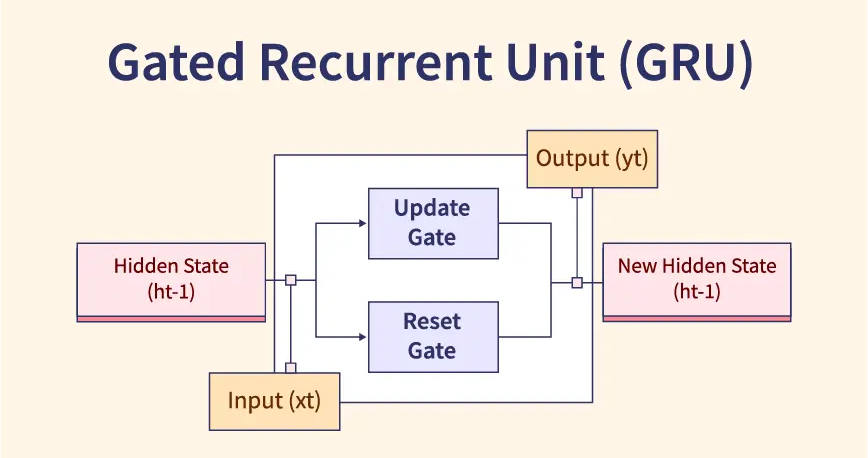
\includegraphics[width=\linewidth]{images/gru.png}
    \caption{Estrutura da GRU}
    \label{fig:gru}
\end{figure}

\indent A arquitetura de GRUs inclui duas portas principais: a porta de atualização e a porta de reinicialização, as quais permitem com que a rede controle o fluxo de informações de modo eficiente\cite{grum}, preservando, assim, informações relevantes de longo prazo e descartando as informações irrelevantes. Isso ocorre devido à presença do \textit{hidden state}, o qual armazena essas informações e carregam elas ao longo de todas as etapas da rede, o que pode ser observado na Figura 1. Isso faz com que esse modelo capture dependências temporais e contextuais importantes para a tarefa de detecção de ódio.

\indent A escolha de GRUs é justificada pela sua eficiência computacional\cite{d2l} e pela sua habilidade de lidar com dependências de longo prazo em sequências de texto, fazendo delas uma ferramenta importante para a tarefa de detecção de ódio. \\

\subsubsection{Bidirectional Long Short-Term Memory}

\indent As redes Long Short-Term Memory (LSTMs) também foram desenvolvidas para superar as limitações das RNNs tradicionais, como o \textit{vanishing gradient} e \textit{exploding gradient}, permitindo a captura de dependências de longo prazo em sequências de dados. Entretanto, ela possui uma variação chamada de Bidirectional LSTM (BiLSTM), a qual estende essa capacidade de processamento da sequência de entrada em ambas as direções: da primeira para a última palavra e da última para a primeira\cite{geeks}, permitindo com que o modelo capture contextos passados e futuros concomitantemente e, consequentemente, oferecendo uma compreensão mais completa do texto.

A arquitetura de um bloco LSTM é composta por células de memória, onde cada célula é responsável por manter informações relevantes ao longo do tempo, controlando o fluxo de informações através de três portas principais: a porta de entrada, a porta de esquecimento e a porta de saída.

\begin{figure}[h!]
    \centering
    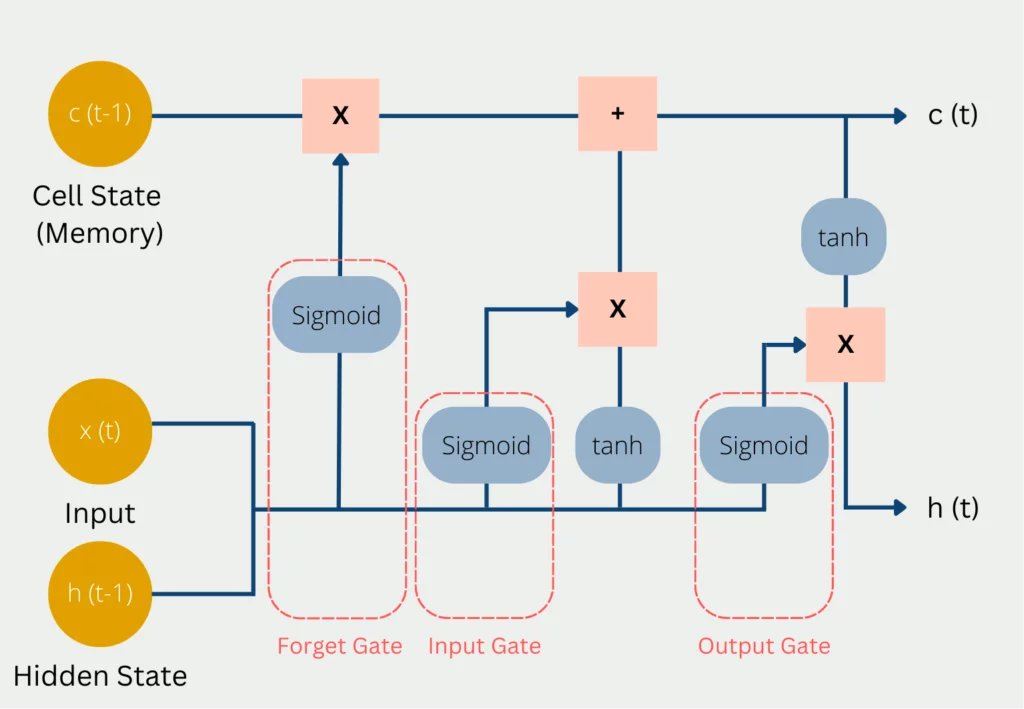
\includegraphics[width=\linewidth]{images/lstm.png}
    \caption{Blocos LSTM}
    \label{fig:exemplo1}
\end{figure}

Na porta de entrada, uma função sigmoide decide quais valores serão atualizados, enquanto uma função tanh cria um vetor de novos valores candidatos para serem adicionados à célula de memória. Já a porta de esquecimento utiliza uma função sigmoide para determinar quais informações da célula de memória anterior serão descartadas. Por fim, a porta de saída, também através de uma função sigmoide decide quais informações da célula de memória serão enviadas para a próxima unidade LSTM e para a saída final \cite{lstms}. A utilização da \textit{cell state} e da \textit{hidden state} objetivam armazenas informações à longo e curto prazo, respectivamente. Esse esquema pode ser visto na Figura 2.

\indent Em uma BiLSTM, a sequência de entrada é processada por duas camadas LSTM distintas: a camada \textit{forward} e a camada \textit{backward}, podendo ser visualizada na Figura 3. A camada \textit{forward} processa essa sequência na direção natural, capturando as independências e informações contextuais que aparecem cronologicamente. Simultaneamente, a camada \textit{backward} processa a mesma sequência de dados, mas na direção oposta, capturando contextos quando os dados são analisados em retrospectiva. Após esses processos, as saídas são combinadas, geralmente por concatenação, para formar uma representação completa em cada ponto da sequência \cite{bilstm}.

\begin{figure}[h!]
    \centering
    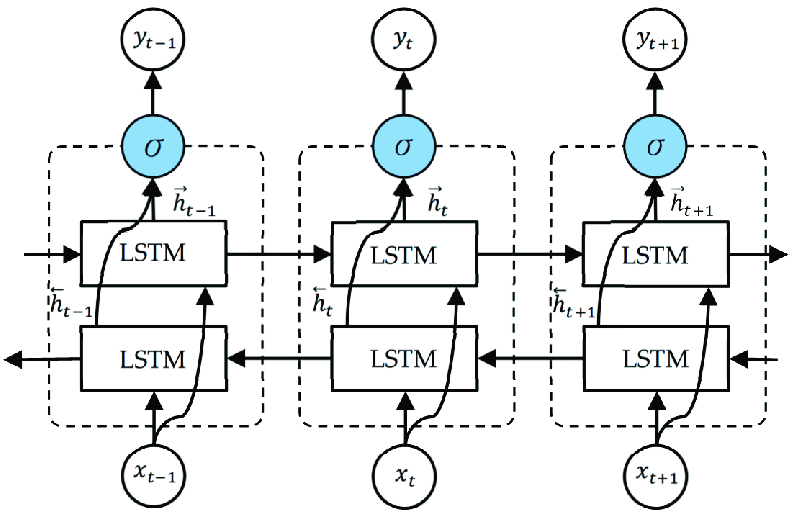
\includegraphics[width=\linewidth]{images/bilstm.png}
    \caption{Estrutura da BiLSTM}
    \label{fig:exemplo2}
\end{figure}

\indent Para esse trabalho, a BiLSTM será útil na identificação de discurso de ódio ao capturar dependências complexas e contextos bidirecionais nos textos, melhorando a robustez do modelo na detecção de conteúdo prejudicial.

\subsection{Transformers}

Os Transformers revolucionaram o campo do Processamento de Linguagem Natural (PLN) ao oferecer uma maneira eficiente, escalar e diferenciada de modelar dependências de longo alcance em dados sequenciais. Diferentemente das Redes Neurais Recorrentes, os Transformers não processam dados de maneira sequencial, o que permite um paralelismo \cite{mama} importante para o treinamento.

\begin{figure}[h!]
    \centering
    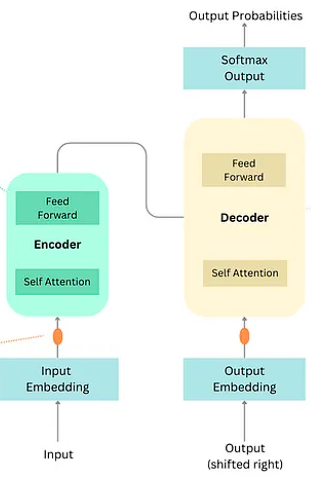
\includegraphics[width=\linewidth]{images/transformer.png}
    \caption{Estrutura geral dos Transformers}
    \label{fig:exemplo3}
\end{figure}

A arquitetura dos Transformers é formada por camadas de atenção e \textit{feed-forward}. A principal inovação dos Transformers é o mecanismo de atenção, especificamente a atenção multi-cabeça, a qual permite com que o modelo foque em diferentes partes da sequência de entrada simultaneamente. Cada camada de atenção é seguida por uma camada \textit{feed-forward} totalmente conectada \cite{trastru}. No codificador, a sequência de entrada é processada por várias dessas camadas de atenção e \textit{feed-forward}, enquanto que no decodificador, a sequência de saída é gerada de forma auto-regressiva, uma palavra por vez, usando informações do codificador através de mecanismos de atenção cruzada. Além disso, o uso de \textit{embeddings} posicionais permite ao modelo incorporar a ordem das palavras na sequência, compensando a falta de processamento sequencial natural das Redes Neurais Recorrentes\cite{tra}. Isso pode ser facilmente visualizado na Figura 4.

A importância dos Transformers para a detecção de discurso de ódio reside em sua capacidade de capturar relações complexas e contextos longos em textos, sendo crucial para identificar nuances e implicitudes que frequentemente caracterizam discursos de ódio.

\subsection{Parâmetros}

Para a realização dos experimentos, vários parâmetros foram testados, incluindo diferentes otimizadores (Adam, SGD e RMSprop), taxas de aprendizado (\textit{learning rate}), número de camadas ocultas (\textit{hidden layers}), taxa de \textit{dropout} e número de cabeças (\textit{num heads}) nos modelos transformer. 

Testar uma variedade de parâmetros é importante para identificar a combinação que resulta no melhor desempenho do modelo, permitindo ajustá-lo a fim de maximizar todas as métricas que analisam o desempenho. A escolha adequada de parâmetros também reduz o tempo de treinamento e melhora a capacidade de generalização do modelo. A seguir, apresentamos a definição de cada um desses parâmetros. \\

\subsubsection{Otimizador}

Os otimizadores são algoritmos usados para ajustar os pesos da rede neural com o objetivo de minimizar a função de perda. Três otimizadores foram testados: Adam, SGD e RMSprop. O otimizador Adam combina as vantagens de dois outros métodos de otimização: AdaGrad e RMSProp, proporcionando uma convergência rápida e eficiente. O SGD (\textit{Stochastic Gradient Descent}) é bastante utilizado por sua simplicidade e eficiência, atualizando os pesos da rede com base em um subconjunto aleatório dos dados de treinamento. O RMSprop, por sua vez, ajusta a taxa de aprendizado para cada parâmetro, dividindo a taxa de aprendizado pelo valor médio dos gradientes recentes, ajudando a manter a estabilidade do treinamento \cite{otm}. \\

\subsubsection{Learning Rate}

A taxa de aprendizado é um hiperparâmetro que controla o quanto os pesos da rede neural são ajustados com base no gradiente estimado. Valores muito altos podem fazer com que o modelo não converja, enquanto que valores muito baixos podem resultar em um treinamento muito lento e possivelmente em um mínimo local ruim \cite{lr}. Testar diferentes taxas de aprendizado ajuda a encontrar um equilíbrio entre velocidade e precisão de convergência. \\

\subsubsection{Número de Camadas Ocultas}

O número de camadas ocultas consiste na quantidade de camadas entre a camada de entrada e a camada de saída em uma rede neural. Mais camadas ocultas podem permitir que a rede capture padrões mais complexos nos dados, mas também podem aumentar o risco de \textit{overfitting} e aumentar o tempo de treinamento \cite{hid}. Testar diferentes números de camadas ocultas ajuda a determinar a arquitetura ideal da rede. \\

\subsubsection{Dropout}

A taxa de \textit{dropout} é uma técnica de regularização utilizada para prevenir \textit{overfitting} em redes neurais, principalmente nos transformers. Durante o treinamento, unidades da rede são desligadas aleatoriamente com uma determinada probabilidade, impedindo que o modelo se torne excessivamente dependente de neurônios específicos, forçando a rede a aprender representações mais robustas e generalizáveis dos dados \cite{dro}. \\

\subsubsection{Número de Cabeças}

O número de cabeças é um parâmetro específico para os transformers, que define quantas sub-representações independentes serão aprendidas em cada camada de atenção multi-cabeça. Mais cabeças permitem que o modelo se concentre em diferentes partes da entrada ao mesmo tempo, melhorando a capacidade da rede de capturar relações complexas entre os tokens de entrada \cite{nca}.


\subsection{Métricas}

Com o intuito de avaliar a eficácia dos modelos de detecção de discurso de ódio em textos, é imprescindível utilizar um conjunto abrangente de métricas que ofereçam uma visão completa do desempenho obtido. Elas foram escolhidas com o objetivo de levar em consideração diversos aspectos dos modelos, como a capacidade do modelo de identificar corretamente as classes, minimizar a quantidade de falsos positivos e falsos negativos e manter um equilíbrio entre precisão e \textit{recall}.

Dessa forma, as métricas selecionadas permitem uma avaliação robusta e confiável dos modelos, proporcionando uma compreensão ampla de seus potenciais e suas limitações em diversos cenários de uso. A seguir, as principais métricas utilizadas são detalhadas:

\begin{enumerate}
    \item Acurácia: A acurácia mede a proporção de previsões corretas entre o total de previsões realizadas \cite{Shwartz}. Em outros termos, é a fração das previsões que o modelo classificou corretamente, incluindo tanto as instâncias positivas quanto as negativas.
    \begin{equation}
    \text{Acur\'{a}cia} = \frac{VP + VN}{VP + FP + VN + FN}
    \end{equation} \\
    
    \item Precisão: A precisão avalia a fração de instâncias positivas classificadas corretamente em relação a todas as instâncias positivas \cite{IF}, sejam elas verdadeiras ou falsas. Ou seja, mensura a capacidade do modelo específico de classificar corretamente as ocorrências positivas.
    \begin{equation}
    \text{Precis\~{a}o} = \frac{VP}{VP + FP}
    \end{equation} \\
    
    \item \textit{Recall}: Também conhecida como revocação ou sensibilidade, \textit{recall} mede a proporção de instâncias positivas que foram classificadas corretamente em relação ao conjunto total de ocorrências positivas \cite{Google}.
    \begin{equation}
    \text{Recall} = \frac{VP}{VP + FN}
    \end{equation} \\
    
    \item F1-Score: F1-score consiste da média harmônica entre a precisão e o \textit{recall}, significando que ele penaliza qualquer valor extremo encontrado, fornecendo, assim, uma medida balanceada do desempenho do modelo \cite{Hicks2022}.
    \begin{equation}
    \text{F1-score} = \frac{2 \cdot (\text{precisão} \cdot \text{recall})}{\text{precisão} +    \text{recall}} 
    \end{equation} 
    
    \begin{equation}
    \text{F1-score} = \frac{2 \cdot VP}{2 \cdot VP + FP + FN}
    \end{equation} \\
    
    \item AUC-ROC: A área sobre curva ROC é uma métrica que avalia a capacidade do modelo em distinguir entre as classes positivas e negativas \cite{medium}. Não há uma fórmula simples e útil para calculá-la, uma vez que ela é calculada numericamente integrando a curva ROC. Entretanto, ela utiliza os parâmetros \textit{True Positive Rate} (TPR) e \textit{False Negative Rate} (FNR):
    \begin{equation}
    \text{TPR} = \frac{VP}{VP + FN}
    \end{equation}
    
    \begin{equation}
    \text{FNR} = \frac{FP}{FP + VN}
    \end{equation} \\
    
\end{enumerate}

\section{Resultados}

Os resultados obtidos ao longo deste trabalho destacam a eficácia dos modelos de redes neurais profundas na detecção de discurso de ódio em textos. A análise detalhada dos dados coletados, combinada com a implementação e treinamento robustos dos modelos, permitiu alcançar um desempenho significativo na identificação de conteúdo prejudicial. Nesta seção, exploramos os resultados dos modelos de Redes Neurais Recorrentes (RNNs) e Transformers. As métricas de desempenho abordadas são discutidas para ilustrar a eficiência de cada modelo. Além disso, são apresentadas as implicações desses resultados para a moderação de conteúdo nas redes sociais e as possíveis melhorias para futuras pesquisas na área.

\subsection{Gated Recurrent Unit}

Primeiramente, é essencial analisar o desempenho dos modelos de Gated Recurrent Unit (GRU) treinados com base nos otimizadores para a detecção do discurso de ódio. O gráfico da Figura 5 apresenta a relação entre a acurácia e o F1-Score dos modelos. Essas duas métricas foram escolhidas para compor os gráficos da seção, pois esta envolve a precisão e o \textit{recall}, outras métricas importantes utilizadas para a análise dos modelos, enquanto que aquela representa o desempenho geral dos modelos.

\begin{figure}[h!]
    \centering
    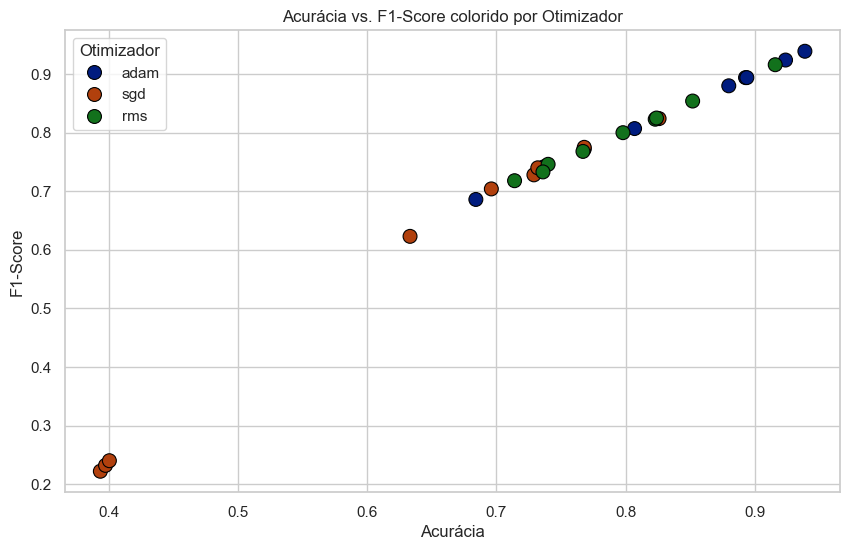
\includegraphics[width=\linewidth]{images/gru-otimizador.png}
    \caption{Acurácia vs F1-Score por Otimizador}
    \label{fig:exemplo4}
\end{figure}

Analisando-o, é possível observar que os modelos otimizados com Adam geralmente apresentam melhores resultados, com acurácia e F1-Score mais elevados em comparação com SGD e RMSprop. A maioria dos pontos relacionados ao Adam está concentrada na parte inferior do gráfico, indicando um bom desempenho. Por outro lado, os modelos otimizados com SGD (\textit{Stochastic Gradient Descent}) mostram maior variabilidade, com muitos pontos distribuídos na parte inferior do gráfico, sugerindo um desempenho menos consistente. Os modelos com RMSprop situam-se entre os outros, apresentando desempenho intermediário.

Através dessa análise de otimizadores, é possível concluir que Adam é o otimizador mais eficiente para os modelos GRU no contexto da detecção do discurso de ódio. Sua capacidade de ajustar os pesos de forma mais eficaz resulta em uma melhor performance global.

Além disso, também é possível realizar uma análise baseada nas taxas de aprendizado diferentes utilizadas nos modelos GRUs treinados, o que pode ser facilmente visualizado no gráfico da Figura 6.

\begin{figure}[h!]
    \centering
    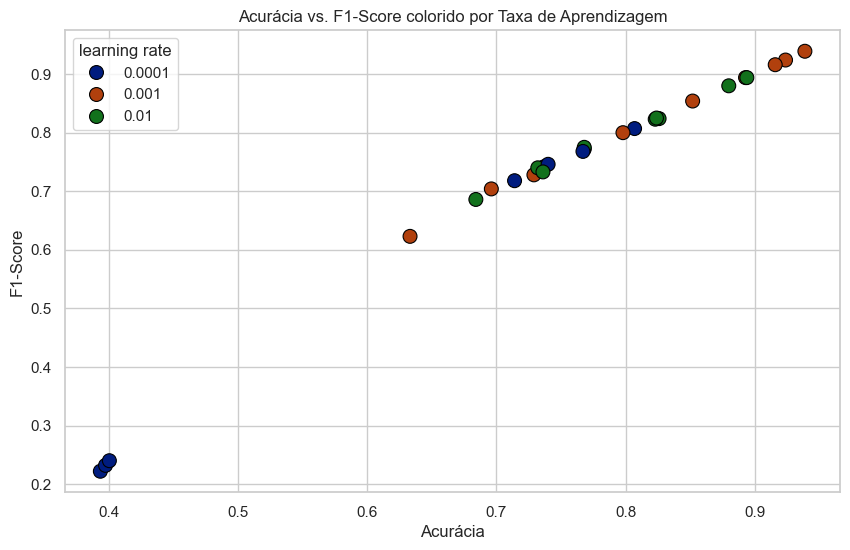
\includegraphics[width=\linewidth]{images/gru-lr.png}
    \caption{Acurácia vs F1-Score por taxas de aprendizado}
    \label{fig:exemplo5}
\end{figure}

Os resultados mostram que a taxa de aprendizado de 0,001 tende a ser a mais eficaz, resultando em modelos com métricas elevadas e consistentes. A taxa de 0,0001, embora tenha produzido alguns modelos de bom desempenho, apresenta maior variabilidade e alguns modelos com desempenho inferior, além de que, já que esse número é muito baixo, os modelos com essa \textit{learning rate} demoram muito para serem treinados e, perceptivelmente, não é um bom investimento. A taxa de 0,001 também representou resultados similares, com alguns modelos com bom desempenho, mas também possuindo alta instabilidade, com vários modelos apresentando desempenho bem abaixo do esperado.

Isso indica que a taxa de aprendizagem de 0,001 é a mais adequada para o desenvolvimento de GRUs para a detecção do discurso de ódio, proporcionando um equilíbrio ideal entre a estabilidade do treinamento e a capacidade do modelo de aprender padrões complexos presentes nos dados.

Experimentos testando diferentes números de \textit{hidden layers} também foram realizados, contudo nenhuma conclusão pode ser afirmada devido à enorme variabilidade de resultados quando esse fator foi levado em consideração, fazendo com que ele não seja tão crucial quanto os outros parâmetros para um bom desempenho do modelo.

Os resultados apresentados indicam que tanto a escolha do otimizador quanto a taxa de aprendizagem são fatores importantes que afetam significativamente o desempenho dos modelos de GRU treinados para a detecção do discurso de ódio. A combinação do otimizador Adam com uma \textit{learning rate} de 0,001 resultou nos melhores desempenhos, fazendo com que o modelo treinado com base nessa configuração capture de forma eficaz os padrões complexos nos dados utilizados para a detecção do discurso de ódio.

\subsection{Bidirectional Long Short-Term Memory}

Primeiramente, é essencial analisar o desempenho dos modelos de Bidirectional Long Short-Term Memory (BiLSTM) treinados com base nos otimizadores para a detecção do discurso de ódio. O gráfico da Figura 7 apresenta a relação entre a acurácia e o F1-Score dos modelos. Essas duas métricas foram escolhidas para compor os gráficos da seção, pois esta envolve a precisão e o \textit{recall}, outras métricas importantes utilizadas para a análise dos modelos, enquanto que aquela representa o desempenho geral dos modelos.

\begin{figure}[h!]
    \centering
    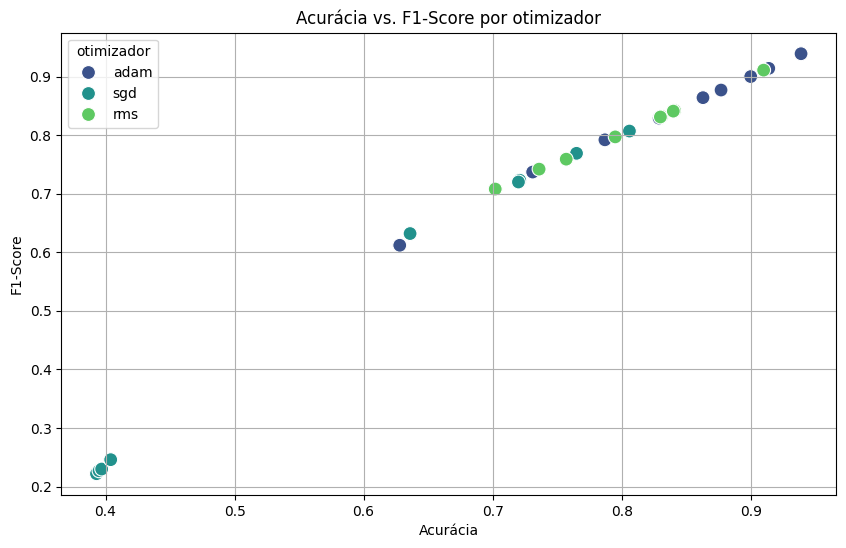
\includegraphics[width=\linewidth]{images/bilstm-otimizador.png}
    \caption{Acurácia vs F1-Score por Otimizador}
    \label{fig:exemplo4}
\end{figure}

Analisando-o, é possível observar que os modelos otimizados com Adam geralmente apresentam melhores resultados, com acurácia e F1-Score mais elevados em comparação com SGD e RMSprop. A maioria dos pontos relacionados ao Adam está concentrada na parte superior do gráfico, indicando um bom desempenho. Por outro lado, os modelos otimizados com SGD (\textit{Stochastic Gradient Descent}) mostram maior variabilidade, com muitos pontos distribuídos na parte inferior do gráfico, sugerindo um desempenho menos consistente. Os modelos com RMSprop situam-se entre os outros, apresentando desempenho intermediário.

Através dessa análise de otimizadores, é possível concluir que Adam é o otimizador mais eficiente para os modelos BiLSTM no contexto da detecção do discurso de ódio. Sua capacidade de ajustar os pesos de forma mais eficaz resulta em uma melhor performance global.

Além disso, também é possível realizar uma análise baseada nas taxas de aprendizado diferentes utilizadas nos modelos BiLSTM treinados, o que pode ser facilmente visualizado no gráfico da Figura 6.

\begin{figure}[h!]
    \centering
    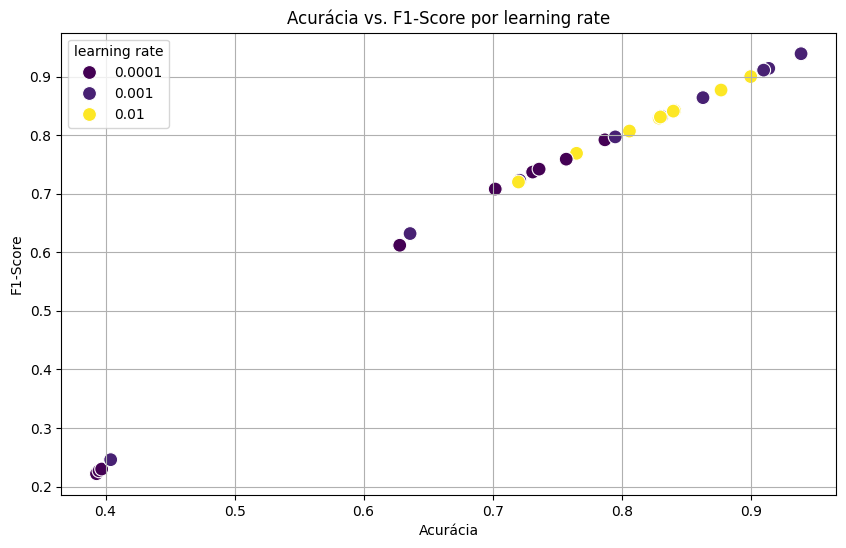
\includegraphics[width=\linewidth]{images/bilstm-lr.png}
    \caption{Acurácia vs F1-Score por taxas de aprendizado}
    \label{fig:exemplo5}
\end{figure}

Os resultados mostram que a taxa de aprendizado de 0,001 tende a ser a mais eficaz, resultando em modelos com métricas elevadas e consistentes. A taxa de 0,0001, embora tenha produzido alguns modelos de bom desempenho, apresenta maior variabilidade e alguns modelos com desempenho inferior, além de que, já que esse número é muito baixo, os modelos com essa \textit{learning rate} demoram muito para serem treinados e, perceptivelmente, não é um bom investimento. A taxa de 0,001 também representou resultados similares, com alguns modelos com bom desempenho, mas também possuindo alta instabilidade, com vários modelos apresentando desempenho bem abaixo do esperado.

Isso indica que a taxa de aprendizagem de 0,001 é a mais adequada para o desenvolvimento de BiLSTMs para a detecção do discurso de ódio, proporcionando um equilíbrio ideal entre a estabilidade do treinamento e a capacidade do modelo de aprender padrões complexos presentes nos dados.

Experimentos testando diferentes números de \textit{hidden layers} também foram realizados, contudo nenhuma conclusão pode ser afirmada devido à enorme variabilidade de resultados quando esse fator foi levado em consideração, fazendo com que ele não seja tão crucial quanto os outros parâmetros para um bom desempenho do modelo.

Os resultados apresentados indicam que tanto a escolha do otimizador quanto a taxa de aprendizagem são fatores importantes que afetam significativamente o desempenho dos modelos de BiLSTM treinados para a detecção do discurso de ódio. A combinação do otimizador Adam com uma \textit{learning rate} de 0,001 resultou nos melhores desempenhos, fazendo com que o modelo treinado com base nessa configuração capture de forma eficaz os padrões complexos nos dados utilizados para a detecção do discurso de ódio.

\subsection{Transformers}

Lorem ipsum dolor sit amet, consectetur adipiscing elit. Cras elementum tempor mauris, eu tempor quam. Vestibulum hendrerit scelerisque ante, non maximus dui ullamcorper vitae. Aliquam id lacus augue. Nullam sed convallis mauris. In convallis eros ut efficitur commodo. Mauris mollis odio sem, id finibus lectus maximus viverra. Nunc euismod imperdiet diam, nec gravida eros tincidunt non. In a velit sed ante tristique accumsan. Praesent gravida turpis vel velit lobortis rutrum. Praesent vitae ipsum at ante volutpat iaculis sit amet id purus. Suspendisse neque arcu, vehicula quis nulla non, rhoncus mattis velit. Mauris sit amet eros ut est elementum ullamcorper id ac erat. Vestibulum sodales quam velit, vitae fringilla metus cursus sagittis.

Lorem ipsum dolor sit amet, consectetur adipiscing elit. Cras elementum tempor mauris, eu tempor quam. Vestibulum hendrerit scelerisque ante, non maximus dui ullamcorper vitae. Aliquam id lacus augue. Nullam sed convallis mauris. In convallis eros ut efficitur commodo. Mauris mollis odio sem, id finibus lectus maximus viverra. Nunc euismod imperdiet diam, nec gravida eros tincidunt non. In a velit sed ante tristique accumsan. Praesent gravida turpis vel velit lobortis rutrum. Praesent vitae ipsum at ante volutpat iaculis sit amet id purus. Suspendisse neque arcu, vehicula quis nulla non, rhoncus mattis velit. Mauris sit amet eros ut est elementum ullamcorper id ac erat. Vestibulum sodales quam velit, vitae fringilla metus cursus sagittis.

\subsection{Discussão}

Lorem ipsum dolor sit amet, consectetur adipiscing elit. Cras elementum tempor mauris, eu tempor quam. Vestibulum hendrerit scelerisque ante, non maximus dui ullamcorper vitae. Aliquam id lacus augue. Nullam sed convallis mauris. In convallis eros ut efficitur commodo. Mauris mollis odio sem, id finibus lectus maximus viverra. Nunc euismod imperdiet diam, nec gravida eros tincidunt non. In a velit sed ante tristique accumsan. Praesent gravida turpis vel velit lobortis rutrum. Praesent vitae ipsum at ante volutpat iaculis sit amet id purus. Suspendisse neque arcu, vehicula quis nulla non, rhoncus mattis velit. Mauris sit amet eros ut est elementum ullamcorper id ac erat. Vestibulum sodales quam velit, vitae fringilla metus cursus sagittis.

Lorem ipsum dolor sit amet, consectetur adipiscing elit. Cras elementum tempor mauris, eu tempor quam. Vestibulum hendrerit scelerisque ante, non maximus dui ullamcorper vitae. Aliquam id lacus augue. Nullam sed convallis mauris. In convallis eros ut efficitur commodo. Mauris mollis odio sem, id finibus lectus maximus viverra. Nunc euismod imperdiet diam, nec gravida eros tincidunt non. In a velit sed ante tristique accumsan. Praesent gravida turpis vel velit lobortis rutrum. Praesent vitae ipsum at ante volutpat iaculis sit amet id purus. Suspendisse neque arcu, vehicula quis nulla non, rhoncus mattis velit. Mauris sit amet eros ut est elementum ullamcorper id ac erat. Vestibulum sodales quam velit, vitae fringilla metus cursus sagittis.


\bibliographystyle{IEEEtran}
\bibliography{refs.bib}
\end{document}